\documentclass[border=0.2cm, 12pt]{standalone}
\usepackage{amsmath, amssymb}  % Only necessary math packages
\usepackage{tikz}              % For drawing
\usepackage{helvet}            % Helvetica font
\renewcommand{\familydefault}{\sfdefault} % Sans-serif as default

\begin{document}
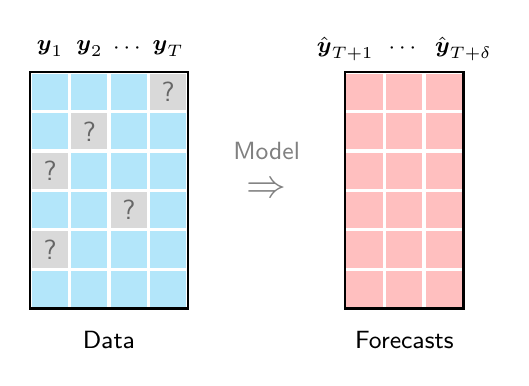
\begin{tikzpicture}[
    % Define styles for consistent formatting
    boxfill/.style={fill=#1, draw=green!40!black, thick},
    gridline/.style={step=0.5, very thick, color=white},
    smalllabel/.style={font=\footnotesize, color=black},
    datalabel/.style={font=\small, color=black},
    question/.style={color=black!60},
    arrowlabel/.style={font=\small, color=gray}
]

% Define coordinates for better maintainability
\newcommand{\locone}{0}
\newcommand{\loctwo}{4}
\newcommand{\boxwidth}{2}
\newcommand{\forecastwidth}{1.5}
\newcommand{\boxheight}{3}
\newcommand{\textoffset}{0.5}

% Main data box
\filldraw [boxfill=cyan!30] (\locone,-\textoffset) rectangle (\locone+\boxwidth,\boxheight-\textoffset);

% Missing data cells (gray)
\foreach \x/\y in {
    0/0, 0/1, 0.5/1.5, 1/0.5, 1.5/2
} {
    \filldraw [fill=gray!30] (\locone+\x,\y) rectangle (\locone+\x+0.5,\y+0.5);
}

% Grid and border
\draw [gridline] (\locone,-\textoffset) grid (\locone+\boxwidth,\boxheight-\textoffset);
\draw [thick] (\locone,-\textoffset) rectangle (\locone+\boxwidth,\boxheight-\textoffset);

% Data labels
\node [smalllabel] at (\locone+0.25,\boxheight-\textoffset+0.3) {$\boldsymbol{y}_1$};
\node [smalllabel] at (\locone+0.75,\boxheight-\textoffset+0.3) {$\boldsymbol{y}_2$};
\node [smalllabel] at (\locone+1.25,\boxheight-\textoffset+0.3) {$\cdots$};
\node [smalllabel] at (\locone+1.75,\boxheight-\textoffset+0.3) {$\boldsymbol{y}_T$};
\node [datalabel] at (\locone+\boxwidth/2,-\textoffset-0.4) {Data};

% Missing value indicators
\foreach \x/\y in {
    0.25/0.25, 0.25/1.25, 0.75/1.75, 1.25/0.75, 1.75/2.25
} {
    \node [question] at (\locone+\x,\y) {?};
}

% Arrow and model indicator
\node [font=\Large, color=gray] at (\locone+3,1) {$\Rightarrow$};
\node [arrowlabel] at (\locone+3,1.5) {Model};

% Forecast box
\filldraw [boxfill=red!25] (\loctwo,-\textoffset) rectangle (\loctwo+\forecastwidth,\boxheight-\textoffset);
\draw [gridline] (\loctwo,-\textoffset) grid (\loctwo+\forecastwidth,\boxheight-\textoffset);
\draw [thick] (\loctwo,-\textoffset) rectangle (\loctwo+\forecastwidth,\boxheight-\textoffset);

% Forecast labels
\node [datalabel] at (\loctwo+\forecastwidth/2,-\textoffset-0.4) {Forecasts};
\node [smalllabel] at (\loctwo,\boxheight-\textoffset+0.3) {$\hat{\boldsymbol{y}}_{T+1}$};
\node [smalllabel] at (\loctwo+0.75,\boxheight-\textoffset+0.3) {$\cdots$};
\node [smalllabel] at (\loctwo+1.5,\boxheight-\textoffset+0.3) {$\hat{\boldsymbol{y}}_{T+\delta}$};

\end{tikzpicture}
\end{document}